\documentclass[10pt,a4paper]{article}
\usepackage[utf8]{inputenc}
\usepackage[slovak]{babel}
\usepackage[T1]{fontenc}
\usepackage{amsmath}
\usepackage{amsfonts}
\usepackage{amssymb}
\usepackage[hidelinks]{hyperref}
\usepackage{graphicx}
\usepackage[]{algorithm2e}
\usepackage[left=2cm,right=2cm,top=2.5cm,bottom=2cm]{geometry}
\author{Dávid Bolvanský}
\begin{document}
\noindent
Projekt: ARM/FITkit3: Zabezpečení dat pomocí 16/32-bit. kódu CRC v IMP 2017/2018\\
Meno a priezvisko: Dávid Bolvanský\\
Login: xbolva00

\section{Cieľ projektu}
	Projekt má za úlohu demonštrovať možnosti zabezpečenia dát 16/32-bitovým kódom CRC na čipe Kinetis K60 z dosky platformy FITkit 3. Projekt bol vypracovaný pomocou Kinetis Design Studio v3.0 a SDK API pre CRC a UART.
	
	
\section{Blok dát a jeho zabezpečenie}
	Za vhodný blok dát bol vybraný reťazec -- text Lorem Ipsum, ktorý sa následne zabezpečoval pomocou CRC16/32. Za \textbf{CRC16} v tomto projekte berieme CRC-16-ANSI/CRC-16-IBM s polynómom \textbf{0x8005} (obrátene 0xA001). \textbf{CRC32} pracuje s polynómom \textbf{0x04C11DB7} (obrátene 0xEDB88320).
	
\section{Výpočet CRC pomocou HW modulu Cyclic Redundancy Check}
	Interakcia s CRC modulom je vykonávaná pomocou SDK API určených na prácu s CRC modulom. V štruktúre \textbf{crc\_config\_t} bolo potrebné nastaviť požadaný polynóm a počiatnú seed hodnotu. Pomocou funkcie \textbf{CRC\_Init} dôjde k inicializácii CRC modulu. Pomocou funkcie \textbf{CRC\_WriteData} zapíšeme dáta na zabezpečenie. Následne, pomocou funkcie \textbf{CRC\_Get16bitResult} / \textbf{CRC\_Get32bitResult} získame výsledny kontrólny CRC súčet.
	
\section{Výpočet CRC pomocou polynómu z tabuľky}
	Tabuľka predstavuje optimalizačný mechanizmus výpočtu CRC, keďže obsahuje výpočty, ktoré by sa inak opätovne počítali pre každý bajt reťazca.
	
	Nižšie uvedený pseudokód\footnote{\url{http://www.sunshine2k.de/articles/coding/crc/understanding_crc.html}} bol použitý v projekte a prezentuje použitie tabuľky pri výpočte CRC.
	
	\SetKwInput{KwData}{Vstup}
	\SetKwInput{KwResult}{Výstup}
	
	\begin{algorithm}
		\KwData{Blok dát}
		\KwResult{Vypočítaná hodnota CRC32}
		crc32 $\leftarrow$ SEED
		
		\For{bajt v bloku dát} {
			table\_index $\leftarrow$ (crc32 xor bajt) and 0xFF
			
			crc32 $\leftarrow$ (crc32 shr 8) xor crc32\_table[table\_index]
		}
		crc32 $\leftarrow$ crc32 xor 0xFFFFFFFF
		
		return crc32
	\caption{Pseudokód výpočtu CRC32 pomocou polynómu z tabuľky}
	
	\end{algorithm}
	
	Zdroj CRC16 tabuľky pre polynóm 0x8005: \url{https://github.com/torvalds/linux/blob/master/lib/crc16.c}
	
	Zdroj CRC32 tabuľky pre polynóm 0x04C11DB7: \url{http://www.ipgp.fr/~tuchais/earthworm/v6.3/src/data_sources/naqs2ew/crc32.c}

\newpage

\section{Výpočet CRC pomocou polynómu (základný algoritmus)}
	Základný algoritmus výpočtu je popísaný nasledujúcim pseudokódom\footnote{\url{https://en.wikipedia.org/wiki/Computation_of_cyclic_redundancy_checks}}.
	
	\begin{algorithm}
		\KwData{Blok dát}
		\KwResult{Vypočítaná hodnota CRC}
		crc $\leftarrow$ SEED
		
		\For{bajt v bloku dát} {
			crc $\leftarrow$ crc xor bajt;
			
			\For{$i = 0;\ i < 8;\ i = i + 1$}{
				crc = (crc shr 1) xor (OBRATENY\_POLYNOM and -(crc and 1));
			}
		}
		
		return crc32
		\caption{Pseudokód výpočtu pomocou polynómu}
		
	\end{algorithm}
	
	Tento pseudokód základného algoritmu na výpočet CRC16/32 bol implementovaný v projekte.
	
\section{Overenie správnosti výpočtov CRC}
	Pre zvolený blok dát sme si predvypočítali CRC16/32 hodnoty, ktoré následne porovnávame s hodnotami získali vyššie spomenutými spôsobmi výpočtu CRC.  Následne sme do bloku dát zaniesli jednu / viac chýb a vykonali výpočty a porovnania znova.
	
	Informácie o správnosti vypočítaných hodnôt pre jednotlivé spôsoby výpočtu sú prezentované na terminál pomocou UARTu. Práca s UARTom prebieha taktiež pomocou SDK API funkcií, menovite \textbf{UART\_Init} na inicializáciu UARTu a \textbf{UART\_WriteBlocking} na zápis dát.
	
	\begin{figure}[h!]
		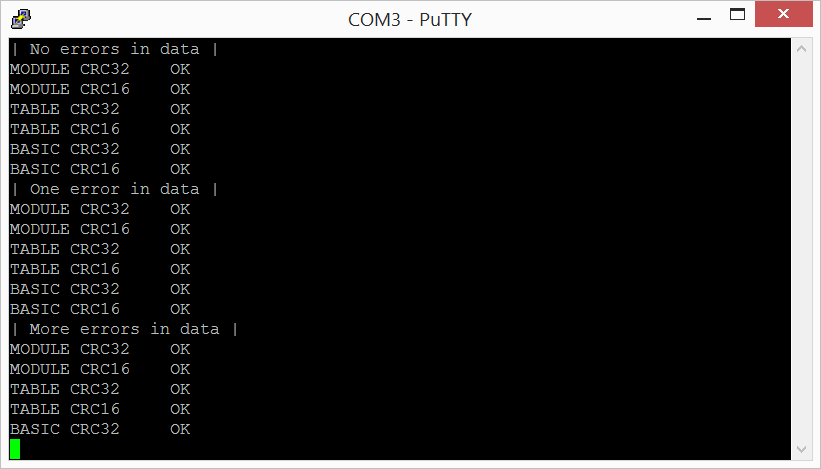
\includegraphics[]{output.png}
		\caption{Výstup aplikácie}
	\end{figure}
	
\newpage

\section{Realizačná a výpočetná režia}
	Obvod hardvérového CRC generátora používa 16/32-bitový programovateľný posuvný register.\footnote{\url{http://cache.freescale.com/files/32bit/doc/ref_manual/K60P144M100SF2V2RM.pdf}}. 

\begin{figure}[h!]
	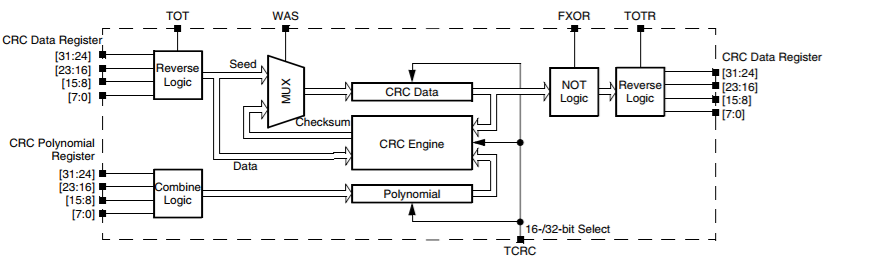
\includegraphics[]{crcmodule.png}
	\caption{Blokový diagram CRC modulu na čipe K60}
\end{figure}


	Podporuje detekciu jednochýb, dvojchýb a väčšiny viacbitových chýb. Hodnota polynómu, seedu je programovateľná. Ponúka vysokorýchlostný výpočet CRC. Voliteľná funkcionalita na transformovanie vstupných dát a výsledku cez transformačný register (pre aplikácie pracujúce s LSB formátom). Možnosť obrátenia (reverzácie) výsledného CRC. 
	
	Režimy MCU ovplyvnujú funkcionalitu CRC modulu -- pri režime nižšieho výkonu, ktorý vypne hodiny, dochádza k prerušeniu CRC výpočtu. Obnoví sa po znovu spustení hodín alebo po systémovom resete, ktorý spôsobí opustenie tohto režimu.
	
	Softvérovým, ale menej efektívnym, riešením, je použitie základného algoritmu výpočtu CRC. Keďže sa počas výpočtu CRC pre každý bajt opakujú niektoré výpočty, vytvorila sa optimalizovaná metóda výpočtu CRC pomocou tabuľky s predvypočítanými hodnotami. Experimenty poukazujú na 5-násobne menej vykonaných inštrukcií v prípade výpočtu CRC pomocou tabuľky oproti základnému algoritmu\footnote{\url{https://barrgroup.com/Embedded-Systems/How-To/CRC-Calculation-C-Code}}.
	
	Softvérové riešenia výpočtu CRC vyžadujú certifikáciu, že spĺňajú požiadavky daného protokolu. Hardvérový CRC modul už tieto podmienky spĺňa. Softvérové riešenie vyžaduje niekoľko stoviek zbernicových cyklov (~700) na spracovanie jedného bajtu cez CRC algoritmu. Hardvérový modul dokáže posunúť bajt do CRC generátora v jednom zbernicovom cykle, čím dochádza k znateľnému zvýšeniu rýchlosti výpočtu. 
	
	Merania na čipe MC9S08AC128 ukazujú, že softvérové riešenie spĺňajúce protokol
	CRC16-CCITT bežiace s rýchlosťou zbernice 20 MHz trvá približne 6,7 sekundy, aby vykonalo kontrolu cyklickým kódom pre 128 KB flash pamäte. Na porovnanie rovnaká kontrola zaberie len 170 ms pri použití hardvérového CRC modulu, čo je výrazne rýchlejšie riešenie\footnote{\url{https://www.nxp.com/docs/en/application-note/AN3795.pdf}}.
	
	Vysoká rýchlosť výpočtu CRC pomocou hardvérového modulu nad softvérovými riešeniami preto predurčuje CRC modul ako ideálneho kandidáta na vykonávanie kontrol cyklickým kódom pri prenosoch dát s minimálnou réžiou.

\end{document}
